\documentclass[tikz,border=7pt]{standalone}
\usepackage{palatino}
\usepackage{amsmath}
\usepackage{amssymb}
\usepackage[none]{hyphenat}
\usepackage{xcolor}
\usetikzlibrary{arrows.meta,calc}

\definecolor{mapink}{HTML}{20252B}
\definecolor{mapgray}{HTML}{707780}
\definecolor{mapline}{HTML}{9199A1}
\definecolor{mapblue}{HTML}{0072B2}
\definecolor{mapbluefill}{HTML}{EAF3FA}
\definecolor{mapgreen}{HTML}{18857A}
\definecolor{mapgreenfill}{HTML}{E9F4F1}
\definecolor{mapred}{HTML}{D55E00}

\begin{document}
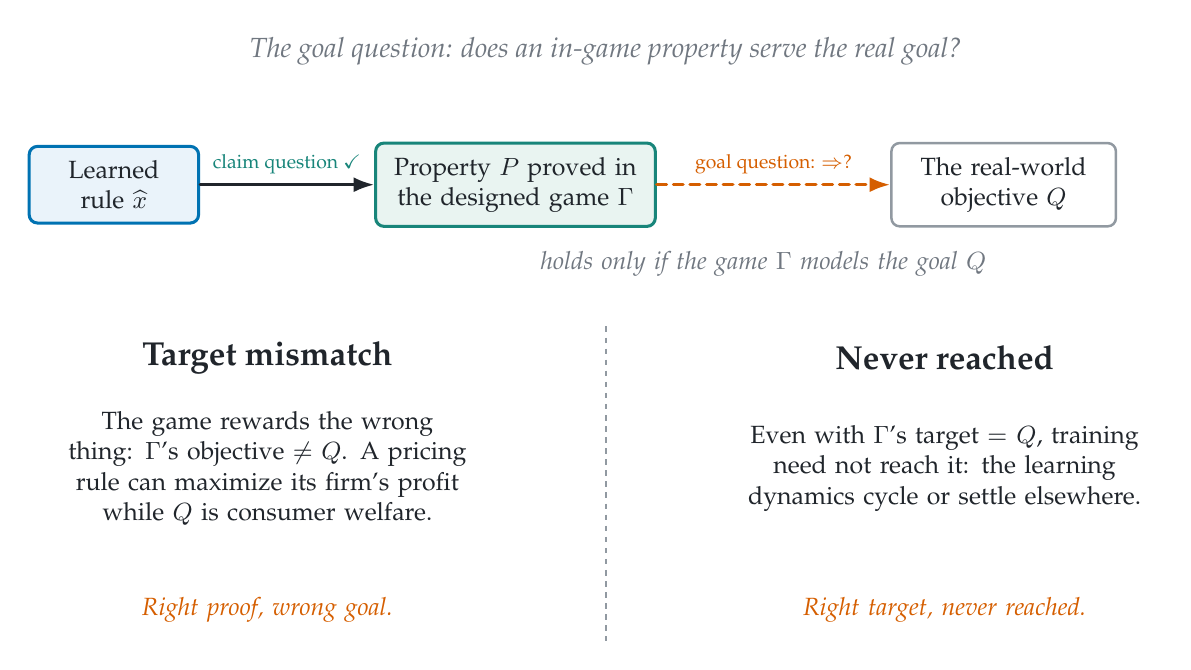
\begin{tikzpicture}[
  font=\rmfamily,
  box/.style={draw=mapline, fill=white, text=mapink, line width=0.9pt,
    rounded corners=3pt, align=center, font=\rmfamily\small, inner sep=5pt},
  bluebox/.style={draw=mapblue, fill=mapbluefill, text=mapink, line width=1.1pt,
    rounded corners=3pt, align=center, font=\rmfamily\small, inner sep=5pt},
  greenbox/.style={draw=mapgreen, fill=mapgreenfill, text=mapink, line width=1.1pt,
    rounded corners=3pt, align=center, font=\rmfamily\small, inner sep=5pt},
  flow/.style={draw=mapink, line width=1.0pt, -{Latex[length=2.6mm,width=1.9mm]}, line cap=round},
  gap/.style={draw=mapred, line width=1.2pt, -{Latex[length=2.6mm,width=1.9mm]},
    line cap=round, dash pattern=on 3.5pt off 2.5pt},
  ptitle/.style={font=\rmfamily\bfseries\large, text=mapink},
  stmt/.style={align=center, font=\rmfamily\small, text=mapink, text width=5.3cm},
  note/.style={align=center, font=\rmfamily\small\itshape},
]

% ===== header =====
\node[font=\rmfamily\itshape, text=mapgray] at (0,4.05)
  {The goal question: does an in-game property serve the real goal?};

% ===== top chain =====
\node[bluebox, text width=1.8cm] (x) at (-6.25,2.35) {Learned rule $\widehat{x}$};
\node[greenbox, text width=3.2cm] (P) at (-1.15,2.35)
  {Property $P$ proved in the designed game $\Gamma$};
\node[box, text width=2.5cm] (Q) at (5.05,2.35) {The real-world objective $Q$};

\draw[flow] (x) -- (P)
  node[midway, above, font=\rmfamily\scriptsize, text=mapgreen] {claim question $\checkmark$};
\draw[gap] (P) -- (Q)
  node[midway, above, font=\rmfamily\scriptsize, text=mapred] {goal question: $\Rightarrow$?};

\node[note, text=mapgray, text width=6.0cm] at (2.0,1.35)
  {holds only if the game $\Gamma$ models the goal $Q$};

% ===== divider =====
\draw[mapline, line width=0.5pt, dash pattern=on 2pt off 2pt] (0,0.55) -- (0,-3.45);

% ===== left failure: target mismatch =====
\node[ptitle] at (-4.3,0.15) {Target mismatch};
\node[stmt] at (-4.3,-1.25)
  {The game rewards the wrong thing: $\Gamma$'s objective $\neq Q$. A pricing rule can
  maximize its firm's profit while $Q$ is consumer welfare.};
\node[note, text=mapred, text width=5.3cm] at (-4.3,-3.05) {Right proof, wrong goal.};

% ===== right failure: never reached =====
\node[ptitle] at (4.3,0.15) {Never reached};
\node[stmt] at (4.3,-1.25)
  {Even with $\Gamma$'s target $=Q$, training need not reach it: the learning dynamics
  cycle or settle elsewhere.};
\node[note, text=mapred, text width=5.3cm] at (4.3,-3.05) {Right target, never reached.};

\end{tikzpicture}
\end{document}
